\documentclass[english,inz,shortabstract]{iithesis}

\usepackage[utf8]{inputenc}
\usepackage{natbib}
\usepackage[nottoc,notlot,notlof]{tocbibind}
\usepackage{graphicx}
\usepackage{enumitem}
\usepackage{hyperref}
\usepackage[justification=centering]{caption}
\usepackage{lipsum}
\usepackage{listings}
\usepackage{color}
\usepackage{todonotes}

\definecolor{codegreen}{rgb}{0,0.6,0}
\definecolor{codegray}{rgb}{0.5,0.5,0.5}
\definecolor{codepurple}{rgb}{0.58,0,0.82}
\definecolor{backcolor}{rgb}{0.90,0.90,0.90}
\definecolor{codered}{RGB}{216, 38, 81}

\lstdefinestyle{mystyle}{
    backgroundcolor=\color{backcolor},
    commentstyle=\color{codegreen},
    keywordstyle=\color{codered},
    numberstyle=\tiny\color{codegray},
    basicstyle=\ttfamily\footnotesize,
    breakatwhitespace=false,
    breaklines=true,
    captionpos=b,
    keepspaces=true,
    numbers=none,
    numbersep=5pt,
    frame=single
}

\lstset{style=mystyle}

\newcommand{\oldrovername}{$\aleph_1$\ }
\newcommand{\rovername}{$\aleph_2$\ }

\newcommand{\todomma}[1]{\todo[author=mma]{#1}}

\englishtitle   {Control software for the \fmlinebreak Aleph2 robot - a Mars rover prototype}
\polishtitle    {Oprogramowanie do kontroli robota\fmlinebreak Aleph2 - prototypu łazika marsjańskiego}
\author         {Błażej Sowa}
\advisor        {dr Marek Materzok}
%\date          {}

\englishabstract{
    The \oldrovername (pron. aleph one) robot is a Mars rover prototype being developed since 2015 by the student research group \textit{Continuum}, operating at the University of Wroclaw. One of the team's most outstanding achievements is 2nd place at the \textit{University Rover Challenge 2017}, where the rover proved itself well performing tasks in the desert in Utah.\\
    The thesis focuses on the implementation of the hardware abstraction layer and the simulation environment created for the successor of the aforementioned robot, \rovername (pron. aleph two). The software is largely based on the use of the Robot Operating System (ROS), ros\_control framework and Gazebo simulator.
}

\polishabstract{
    Robot \oldrovername (czyt. alef jeden) to prototyp łazika marsjańskiego rozwijany od 2015 roku przez koło naukowe \textit{Continuum}, działające na Uniwersytecie Wrocławskim. Do jednych z najwybitniejszych osiągnięć drużyny można zaliczyć 2. miejsce na zawodach \textit{University Rover Challenge 2017}, gdzie łazik bardzo dobrze sprawdził się wykonując zadania na pustyni w Utah.\\    
    Praca skupia się na implementacji warstwy abstrakcji sprzętowej oraz środowisku symulacyjnym stworzonych na potrzeby następcy wyżej wspomnianego robota, \rovername (czyt. alef dwa). Oprogramowanie opiera się w znacznym stopniu na wykorzystaniu Robot Operating System (ROS), frameworku ros\_control i symulatora Gazebo. 
}

\begin{document}

\chapter{Introduction}

\section{Background}
The NASA's \textit{Mars Exploration Rover} mission has inspired various annual robotic competitions for university level students. The challenge is to build a robot that would help early explorers on Mars. 
The \textit{Rover Challenge Series} is a series of such competitions run by the \textit{Mars Society}. Among the most popular are \textit{University Rover Challenge} (hosted since 2007) and \textit{European Rover Challenge} (hosted since 2014).

The tasks on the competitions often include:
\begin{itemize}[itemsep=0pt, parsep=2pt, topsep=0pt]
    \item Navigating through rough terrain
    \item Picking up and transporting objects
    \item Flipping switches on the control panel 
    \item Collecting and examining soil samples
\end{itemize}

\textit{Continuum} (also known as \textit{Team Continuum} or \textit{Continuum Rover Team}) is a student research club from University of Wroclaw whose main focus is to build and improve its Mars rover prototype and compete in the challenges. The team has operated since 2014 and debuted with the \oldrovername (pron. aleph one) robot, scoring 3rd place at \textit{University Rover Challenge 2016} and 2nd place at \textit{University Rover Challenge 2017}.

Now, the team is focused on improving the \rovername rover (Fig. \ref{fig:lazik1} and \ref{fig:lazik2}), which is the next iteration of the \oldrovername robot. 


\begin{figure}[ht]
    \hspace*{\fill}
    \begin{minipage}{.45\textwidth}
      \centering
      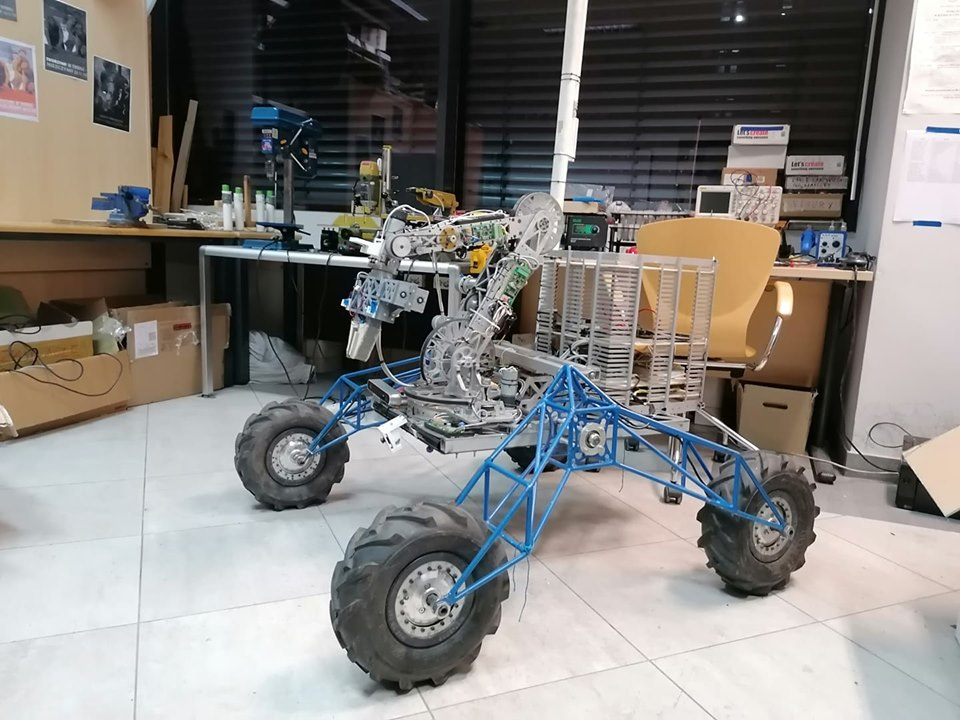
\includegraphics[height=4cm]{img/lazik1.jpg}
      \caption{The current appearance of the \rovername rover}
      \label{fig:lazik1}
    \end{minipage}
    \hfill
    \begin{minipage}{.45\textwidth}
      \centering
      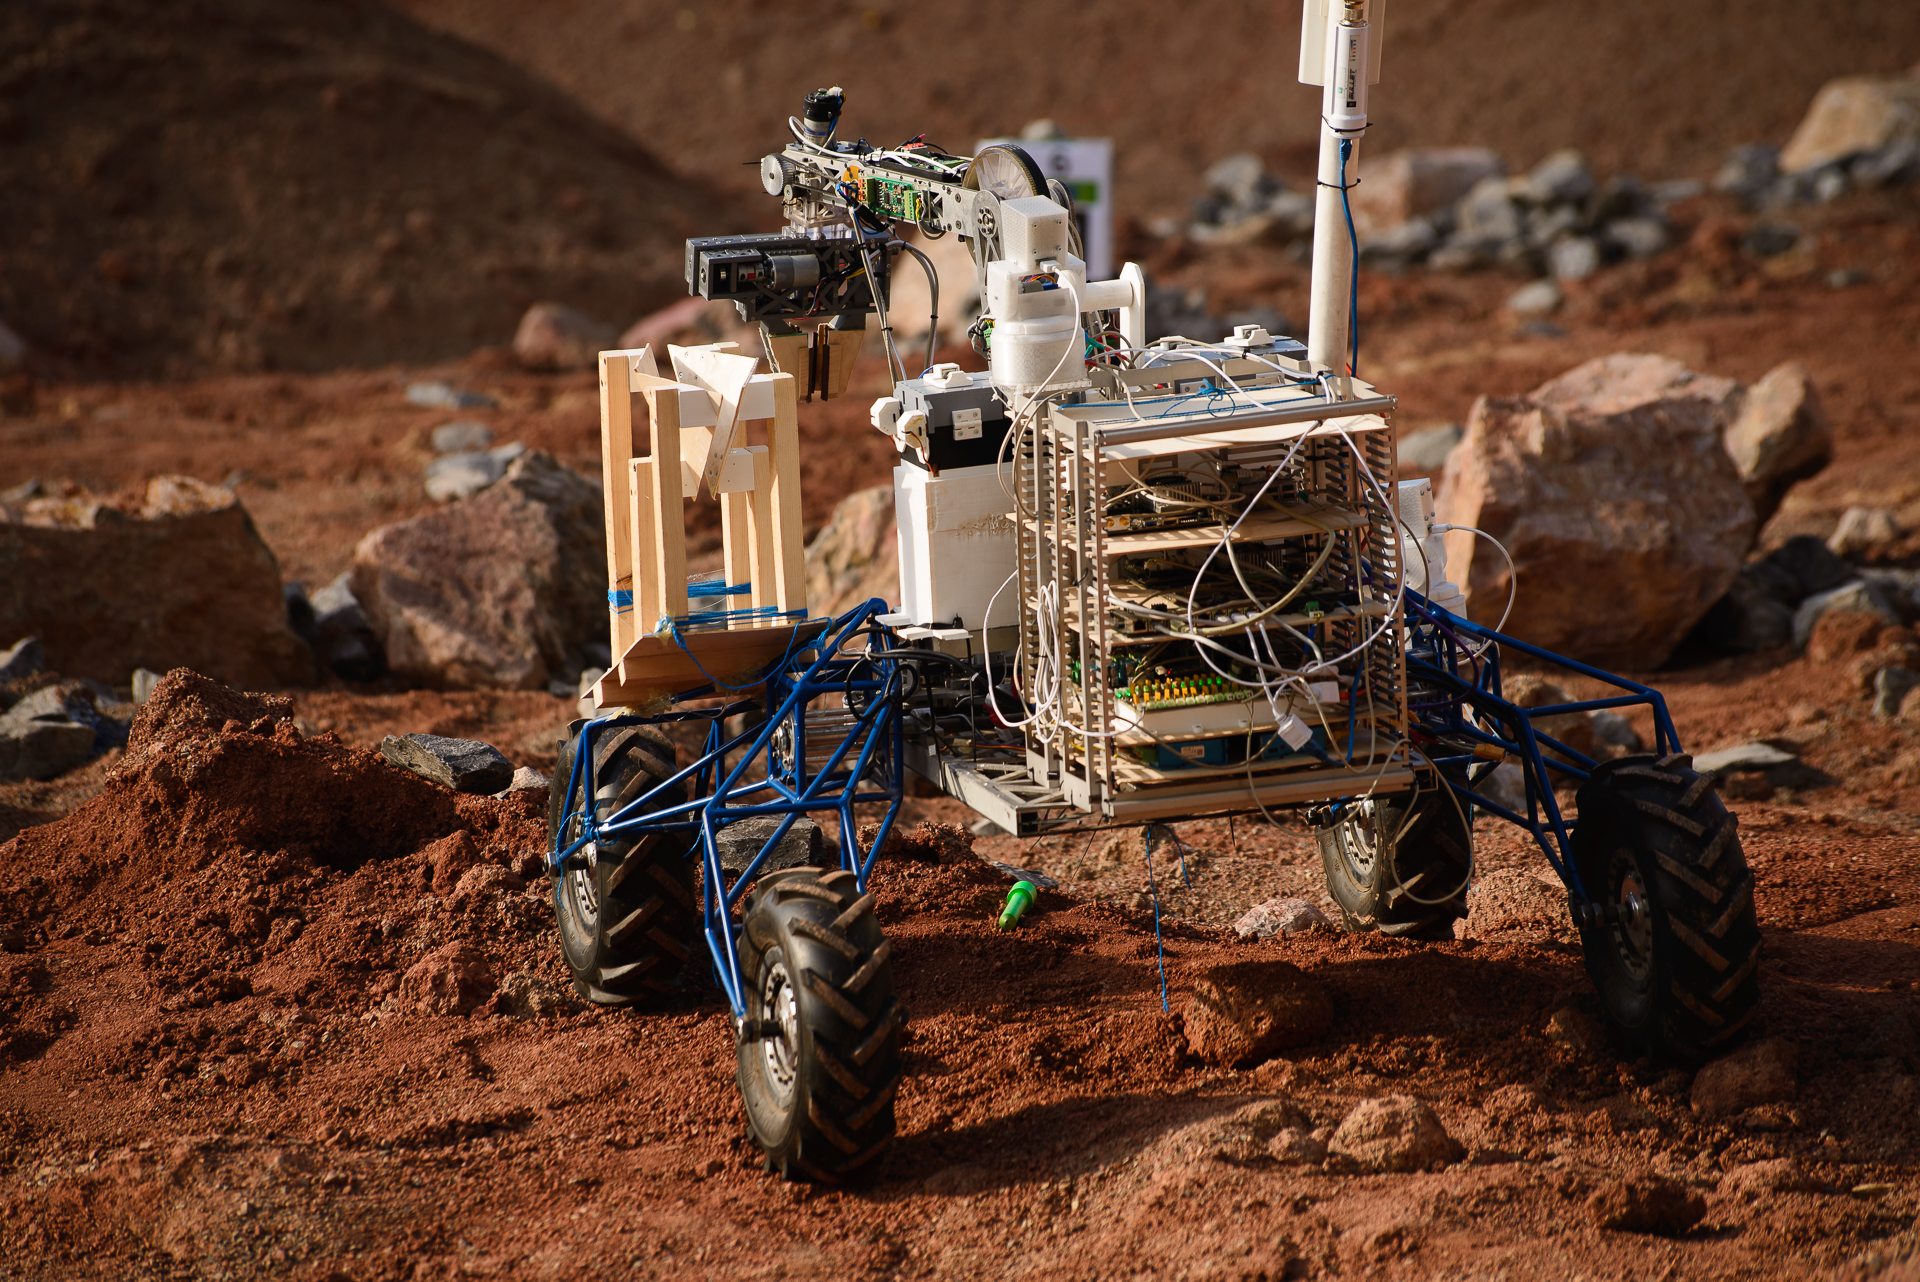
\includegraphics[height=4cm]{img/lazik2.jpg}
      \caption{\rovername performing a task at the \textit{European Rover Challenge 2019}}
      \label{fig:lazik2}
    \end{minipage}
    \hspace*{\fill}
\end{figure}

\section{Motivation}
Although the \oldrovername rover is a well-proven construction piece, its software responsible for robot control and communication with the hardware leaves a lot of room for improvement. The main problems identified are:
\begin{itemize}
    \item \textbf{Unstable implementation} -- the software responsible for the drivetrain often fails to communicate with the motor drivers due to  partial implementation of the communication protocol and various race conditions.
    \item \textbf{Hard-coded configuration} -- all of the configuration (e.g. IDs of the motor drivers, joint names and limits) is embedded into the source code. This makes it needlessly difficult to reconfigure the programs after making changes to other robot subsystems (hardware or software).
    \item \textbf{Lack of abstraction layers} -- the software does not provide any libraries for the implemented controllers or communication protocols. All of these components are placed into single executables. This makes it hard to reuse the code for other purposes.
\end{itemize}
These issues, combined with the passion for robots, were the main reasons that led to the decision of making new control software for the \rovername rover.

\section{Goals}
To address the aforementioned issues with the previous system, a set of design assumptions that the new software has to meet has been defined. The main assumptions include:

\begin{itemize}
    \item \textbf{Extensive use of open source software} -- by relying on widely used and well tested open source projects, the software can become more stable and be developed faster.
    \item \textbf{No hard-coded configuration} -- the programs should not assume much about the hardware they are running on. Instead, they should read the configuration at runtime. The configuration should be well-documented and easily editable.
    \item \textbf{Hardware abstraction layer} -- the software should deliver an abstraction over the hardware it is communicating with by providing interfaces that define its capabilities. This should greatly improve the reusability of the code. 
    \item \textbf{Simulation environment} -- the software should provide the ability to simulate the robot operation in a virtual world. The simulation should be able to run the same set of controllers (ideally, with the same configuration) and provide the same control interfaces as the real robot.
\end{itemize}


\section{Used technologies}
This section describes some of the main concepts of technologies the software is based on, which are essential in order to understand certain parts of this thesis.

    \subsection{ROS}
    \todomma{rozumiem, że to pochylenie oznacza cytowanie? zaznaczyłbym to własnymi kilkoma słowami, może na końcu, może na początku}
    \textit{The Robot Operating System (ROS) is a flexible framework for writing robot software. It is a collection of tools, libraries, and conventions that aim to simplify the task of creating complex and robust robot behavior across a wide variety of robotic platforms.}
    \cite{ros:about}

    This is a brief overview of the concepts related to ROS. A more in-depth information, as well as tutorials, can be found in the documentation \cite{ros:documentation} and in books, such as \cite{ros:mastering}.

    ROS was founded in 2007 by Willow Garage, a robotics research lab and technology incubator devoted to developing hardware and open source software for personal robotics applications \cite{ros:willowgarage}. In 2013, the project was taken over by the Open Source Robotics Foundation (OSRF), a non-profit organization founded by members of the global robotics community.

    It is important to note that ROS in itself is not a real operating system (in the sense of process management) but rather a meta-operating system that runs on top of Unix-based platforms. It provides a layer for communication and management of processes running in a heterogeneous computer cluster (hence the term meta-operating system).

    The basic concepts of ROS include:
    \begin{description}[style=nextline]
        \item [Computation graph] \hfill
        Peer-to-peer network of ROS nodes that are running in a computer cluster.
        \item [Nodes] 
        Processes that perform computation. They can communicate with each other via topics, services or Parameter Server. A typical robot control system will consist of many nodes. For example, one for communication with the hardware, one that performs path planning, one that provides graphical interface, and so on.
        \item [Topics] 
        Named buses over which nodes exchange messages. Nodes do not assume the recipient of the messages they send. Instead, they \textit{publish} to the specified topic. The nodes that want to receive these messages can \textit{subscribe} to the same topic. There is no limit on publishers and subscribers, but only one message type can be sent to one topic.
        \item [Services] 
        Services are similar to topics, but instead of asynchronous stream of data, they allow for synchronous request / reply interactions. They allow one node to call a function that executes in another node and get the result. Two nodes cannot provide the service with the same name.
        \item [Message types]
        For two nodes to successfully communicate via topics or services, a message type definition has to be shared between them. Message types are defined by a simplified description format where a set of fields is listed. Each field contains a name and a type (either a built-in type, an array or another message). Service types use the same description format but both request and reply types are defined.
        \item [Master]
        A program that is essential to run the computation graph. It enables individual nodes to locate each other; keeps track of the running nodes, registered publishers, subscribers, services. The master also provides the Parameter Server.  
        \item [Parameters]
        Globally viewable data entries stored in the Parameter Server that can be retrieved by nodes at runtime. Their primary use is to store static, non-binary data such as configuration for the starting nodes.
        \item [Launch files]
        Describe a set of nodes to run together and parameters to load on the Parameter Server. They provide an easy way to start the whole subsystem by executing only one command. 
        \item [URDF model]
        Unified Robot Description Format (URDF) allows to represent the robot model in a human-readable format, which can be useful in the ROS ecosystem. The elements of the robot, together with their collision, inertial and physical properties, are described by \textit{links}. The connections between \textit{links} (parent and child) are specified by \textit{joints}. (see Fig. \ref{fig:husky}) 
        \item [Packages]
        Main unit for organizing software in ROS. A single package may contain nodes, libraries, message and service type definitions, launch files, URDF models, configuration files and other pieces of software that constitute a useful module. A package also typically defines its dependencies as either other ROS packages or ROS-independent tools, libraries.

    \end{description}

    \begin{figure}[ht]
        \centering
        \captionsetup{margin=2cm}
        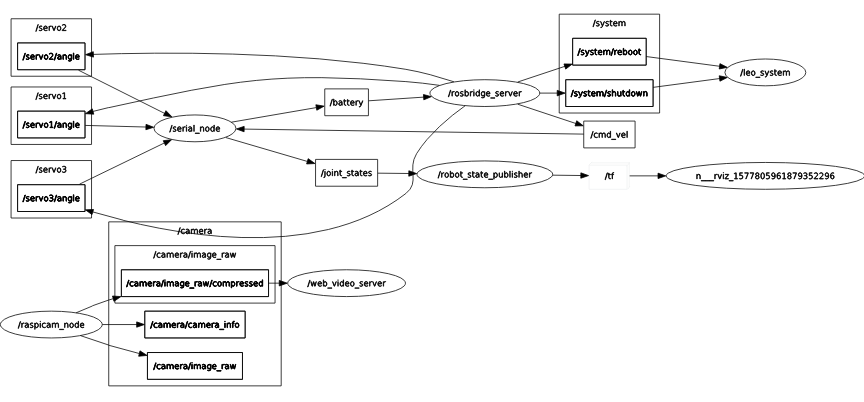
\includegraphics[width=\textwidth]{img/rqt_graph.png}
        \caption{An example visualization of ROS computation graph, created with  \href{http://wiki.ros.org/rqt_graph}{rqt\_graph} tool.}
        \label{fig:ros_graph}
    \end{figure}

    \begin{figure}[ht]
        \centering
        \captionsetup{margin=1cm}
        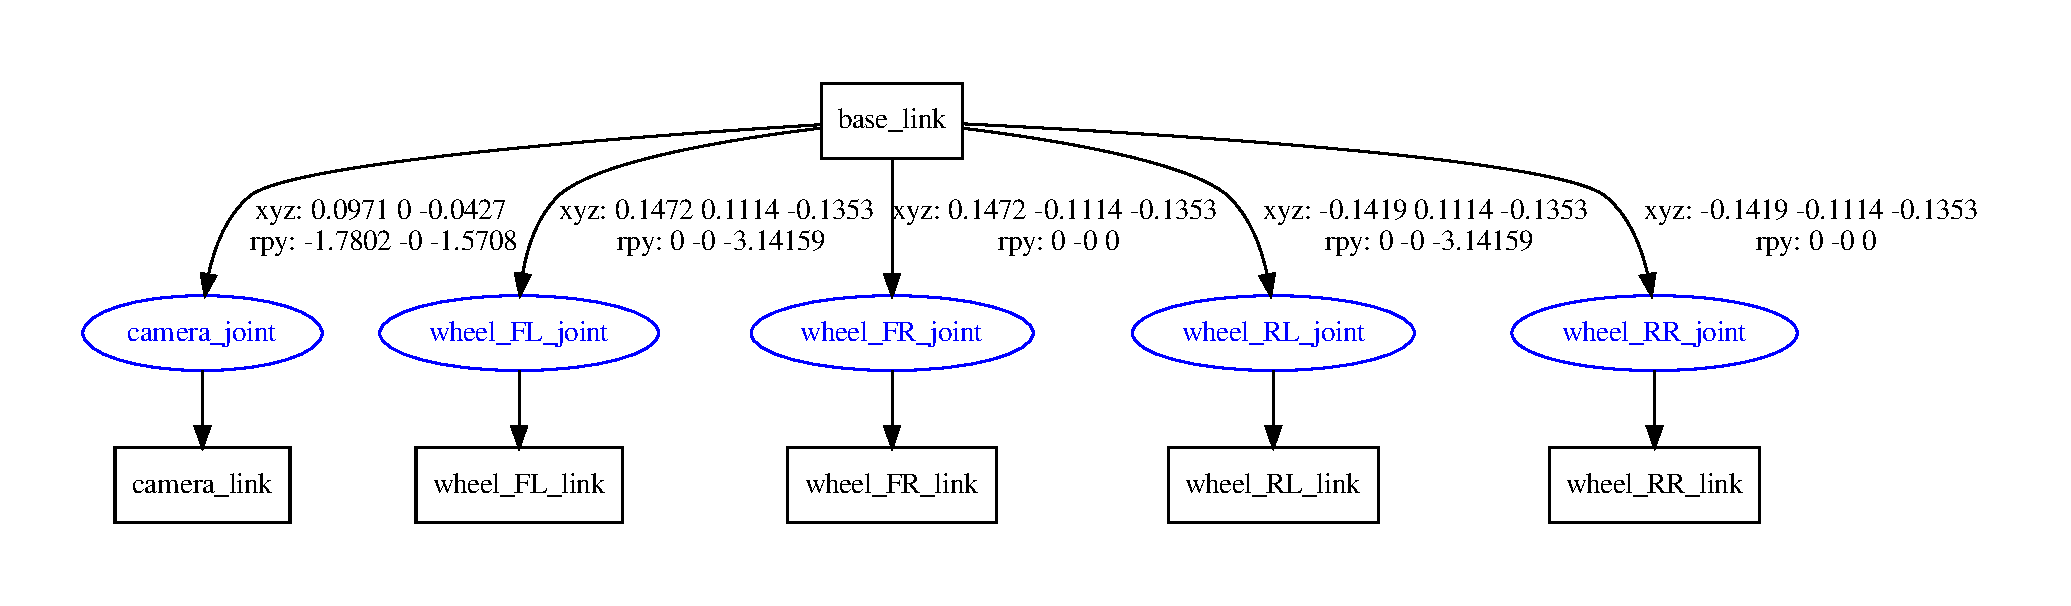
\includegraphics[width=\textwidth]{img/leo_description.pdf}
        \caption{An example visualization of URDF model of four-wheeled robot with a camera, created with \href{http://wiki.ros.org/urdf\#Visualization}{urdf\_to\_graphviz} tool. Black rectangles represent links and blue ovals represent joints.}
        \label{fig:husky}
    \end{figure}

\pagebreak

        \subsubsection{Built-in tools}
        Apart from the communication libraries, the core ROS packages provide many useful utilities, such as command line tools:

        \begin{itemize}[itemsep=0pt, parsep=2pt, topsep=0pt]
            \item \textbf{roscore} -- starts ROS Master, Parameter Server and \href{http://wiki.ros.org/rosout#rosout-1}{rosout} logging node,
            \item \textbf{rosrun} -- runs a node located in an arbitrary package,
            \item \textbf{roslaunch} - launches a set of nodes specified in a launch file, starts roscore if it is not running already,
            \item \textbf{rosnode} -- lists and prints information about running nodes, pings or kills a specified node,
            \item \textbf{rostopic} -- lists and prints information about active topics, displays messages published on a specified topic or publishes on one by itself,
            \item \textbf{rosservice} -- lists and prints information about the advertised services, calls a service and displays the response,
            \item \textbf{rosdep} -- downloads and installs the dependencies of a given package.
        \end{itemize}
        They also provide graphical tools:

        \begin{itemize}[itemsep=0pt, parsep=2pt, topsep=0pt]
            \item \textbf{RQt} -- a framework for GUI applications in ROS. It enables development of Qt-based widgets that can communicate with other nodes running in the system. The base plugins provide many useful functions, such as publishing messages, displaying log messages, plotting data published on topics, visualizing the computation graph and many others,
            \item \textbf{RViz} -- a 3D visualization tool for ROS. It provides plugins for displaying various things that the robot perceives, such as current state of the joints, camera images, data from the sensors, computed localization, occupancy map and many more. It can also be used to interact with the robot via, for example, navigation goal publishing or motion planning execution (see Fig. \ref{fig:rviz_pr2}).
        \end{itemize}

        \begin{figure}[ht]
            \centering
            \captionsetup{margin=2cm}
            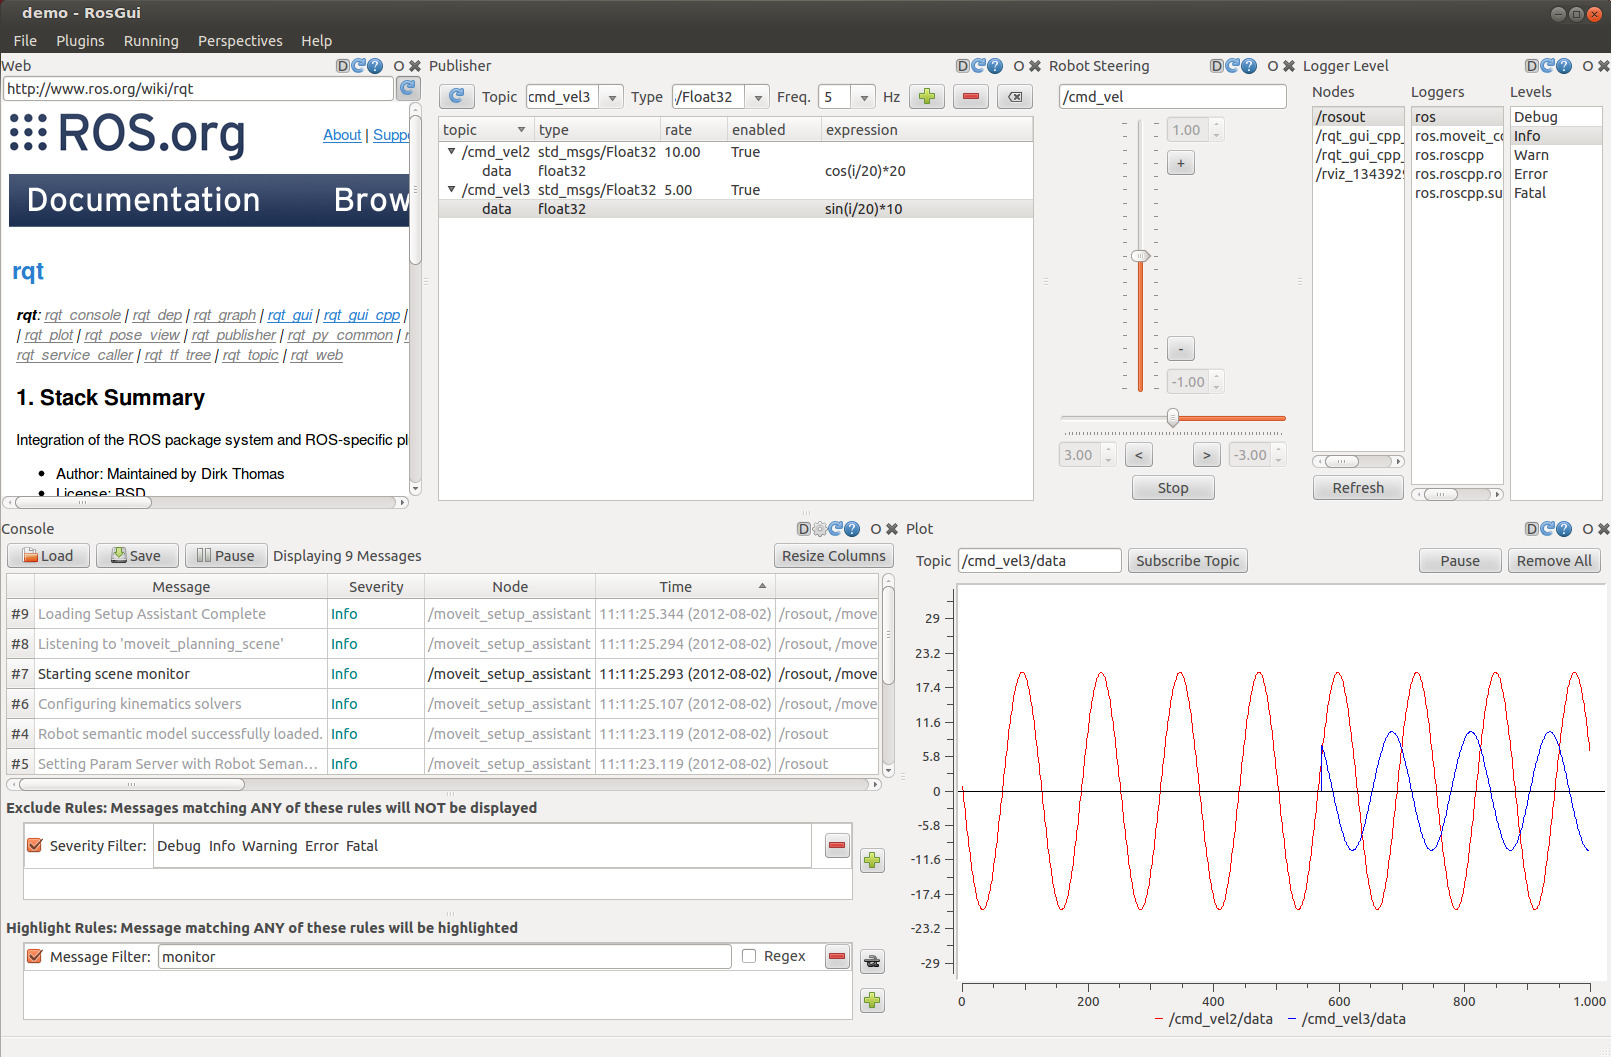
\includegraphics[height=6cm]{img/rqt.png}
            \caption{An example screenshot of RQt (Source: \cite{ros:rqt})}
            \label{fig:rqt}
        \end{figure}

\pagebreak

        \begin{figure}[ht]
            \centering
            \captionsetup{margin=2cm}
            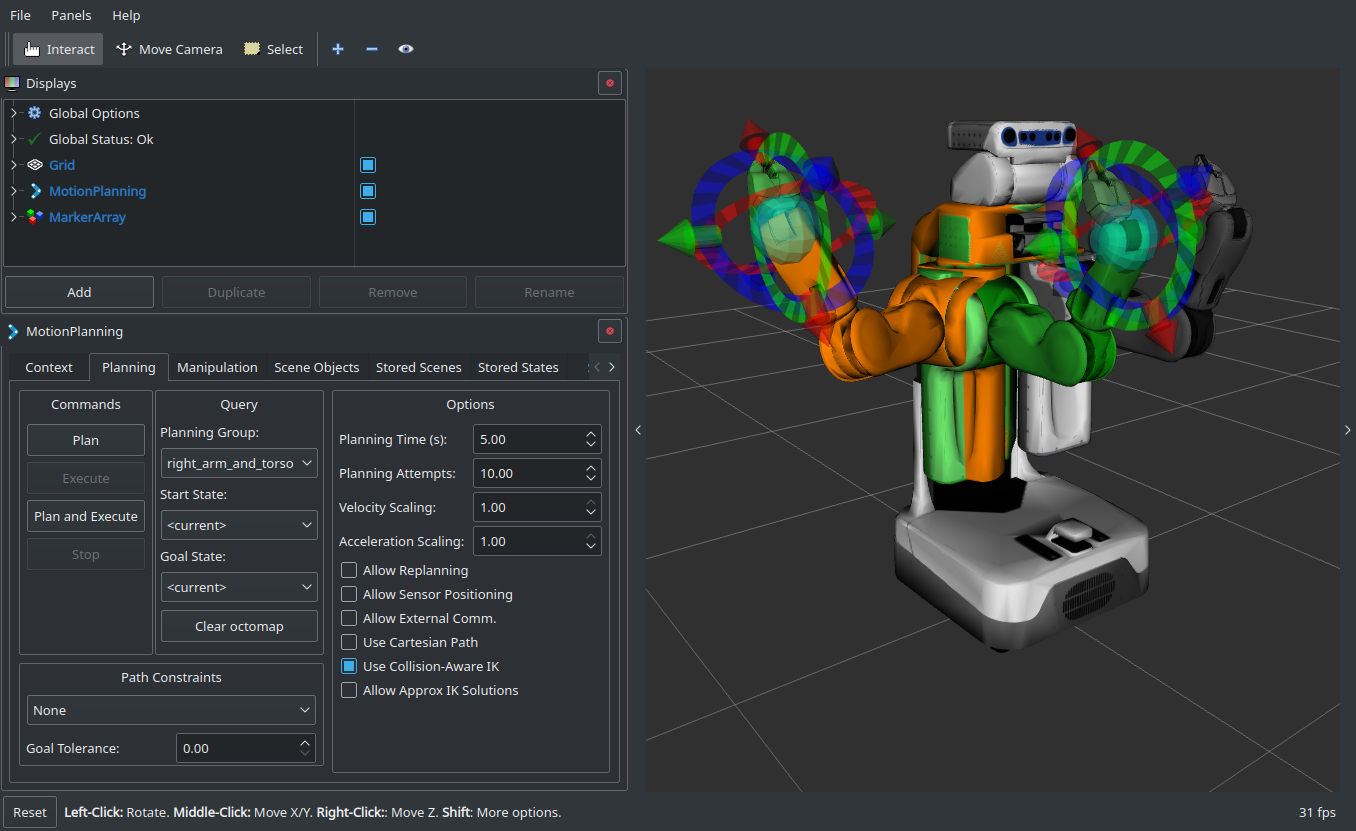
\includegraphics[height=6cm]{img/rviz_pr2.png}
            \caption{RViz utilizing motion planning plugin to move the joints on the PR2 robot}
            \label{fig:rviz_pr2}
        \end{figure}

    \subsection{ros\_control}
    
    \textit{The ros\_control framework provides the capability to implement and manage robot controllers with a focus on both real-time performance and sharing of controllers in a robot-agnostic way.} 
    \cite{ros_control:paper}
    
    \textsf{ros\_control} (also referred as \textsf{ROS control}) was developed as a hardware independent version of \textsf{pr2\_controller\_manager}, which is a framework specific to the PR2 robot. Its core functionality can be summarized by the following components:

    \begin{description}[style=nextline]
        \item [Hardware interfaces]
        Provide a standardized way for communication between controllers and the hardware abstraction layer by sharing resources across them. The most common hardware interfaces include: state interface (for getting the current joint state) and command interfaces (for sending command to the joints, such as effort, velocity or position commands).   
        \item [RobotHW]
        A base class for abstracting custom robot hardware. It provides functions to register and manage hardware interfaces and performs resource conflict checking. To implement a hardware abstraction layer for a robot, the user has to write a derived class that looks similar to this:
        \lstinputlisting[language=C++]{lst/robot_hw.lst}
        \item [Controllers]
        Communicate with the hardware abstraction layer by accessing resources that are shared through hardware interfaces. Some example controller types available in \textsf{ros\_control} include:
            \begin{itemize}
                \item \textsf{joint\_state\_controller/JointStateController} - reads joint states and publishes them on a ROS topic; requires state interface,
                \item \textsf{velocity\_controllers/JointVelocityController} - listens for velocity commands and forwards them to the hardware abstraction layer; requires velocity interface
                \item \textsf{effort\_controllers/JointPositionController} - listens for position commands and forwards effort commands to the hardware abstraction layer; uses a closed-loop controller to get to joint to the specified position; requires effort and state interfaces
            \end{itemize}
        \item [Controller Manager]
        Is responsible for managing the life cycle of the controllers. Provides its functionality through ROS services. It allows to list, load, unload, start or stop controllers. 
        \begin{figure}[ht]
            \centering
            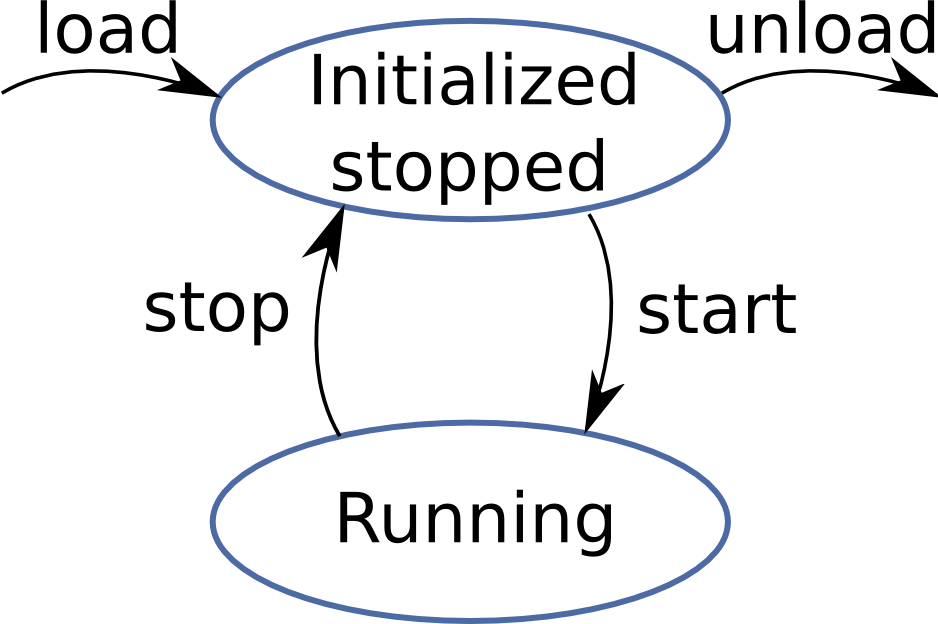
\includegraphics[height=3cm]{img/controller_life.png}
            \caption{Life cycle of a controller (Source: \cite{ros_control:cm_wiki})}
            \label{fig:controller_life}
        \end{figure}

    \end{description}

% \pagebreak
    
    \begin{figure}[ht]
        \centering
        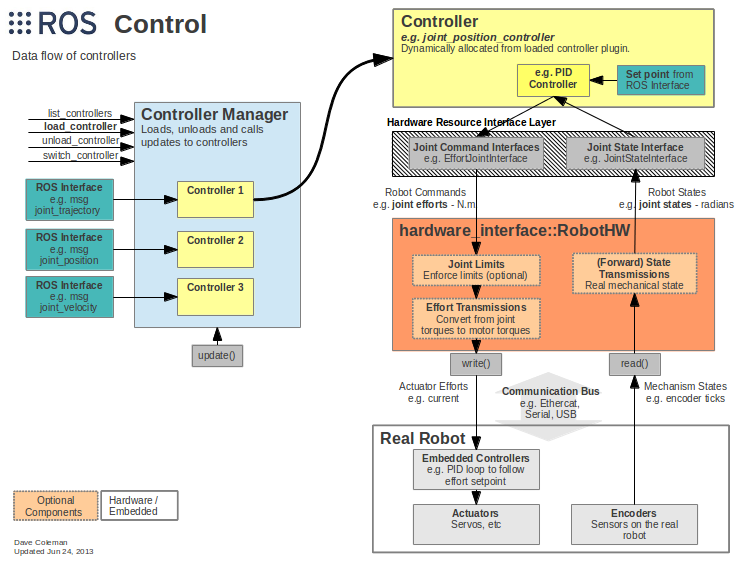
\includegraphics[width=\textwidth]{img/ros_control.png}
        \caption{ROS control overview (Source: \cite{ros_control:wiki})}
        \label{fig:ros_control}
    \end{figure}

    \subsubsection{Control loop}
    After writing the hardware abstraction layer for the robot, the user has to implement a control loop that utilizes the Controller Manager, in order to be able to load some controllers. A sample control loop may look similar to this:

    \lstinputlisting[language=C++]{lst/control_loop.lst}

    \subsection{Gazebo}
    Gazebo provides an open-source 3D simulation environment, mainly for simulating robots. It incorporates a high-performance physics engines, such as Open Dynamics Engine (ODE), Bullet, Dynamic Animation and Robotics Toolkit (DART), etc. and supplies a realistic rendering of the environment. It can model robot behavior, as well as, various sensors, such as cameras, laser range finders, IMU, GPS.

    Gazebo uses its own Simulation Description Format (SDF) to describe a simulation environment (the robots and the world they are moving in), but can also spawn URDF models at runtime. The URDF models need to have physical properties defined (mass, inertia, friction, etc.) and can use gazebo-specific tags to describe additional properties used in simulation.

    \begin{figure}[ht]
        \centering 
        \captionsetup{margin=2.5cm} 
        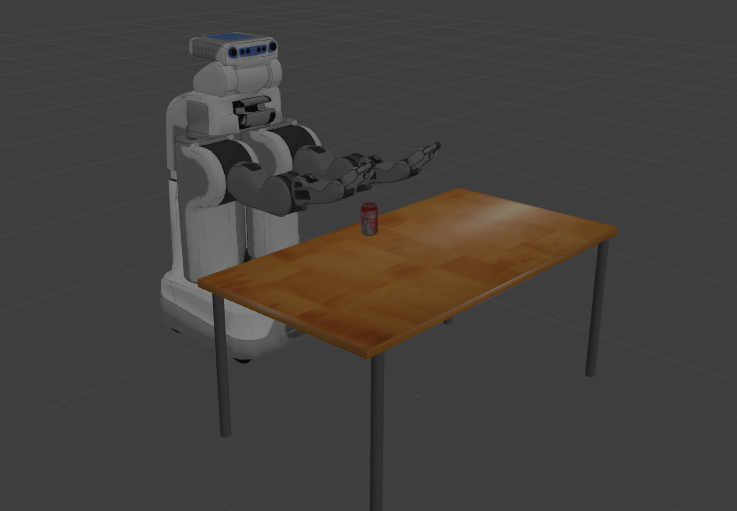
\includegraphics[height=8cm]{img/gazebo_pr2.png}
        \caption{An example simulation of the PR2 robot for testing object grasp operation}
        \label{fig:gazebo_pr2}
    \end{figure}

    \subsubsection{ROS and ros\_control integration}
    

    \begin{figure}[ht]
        \centering
        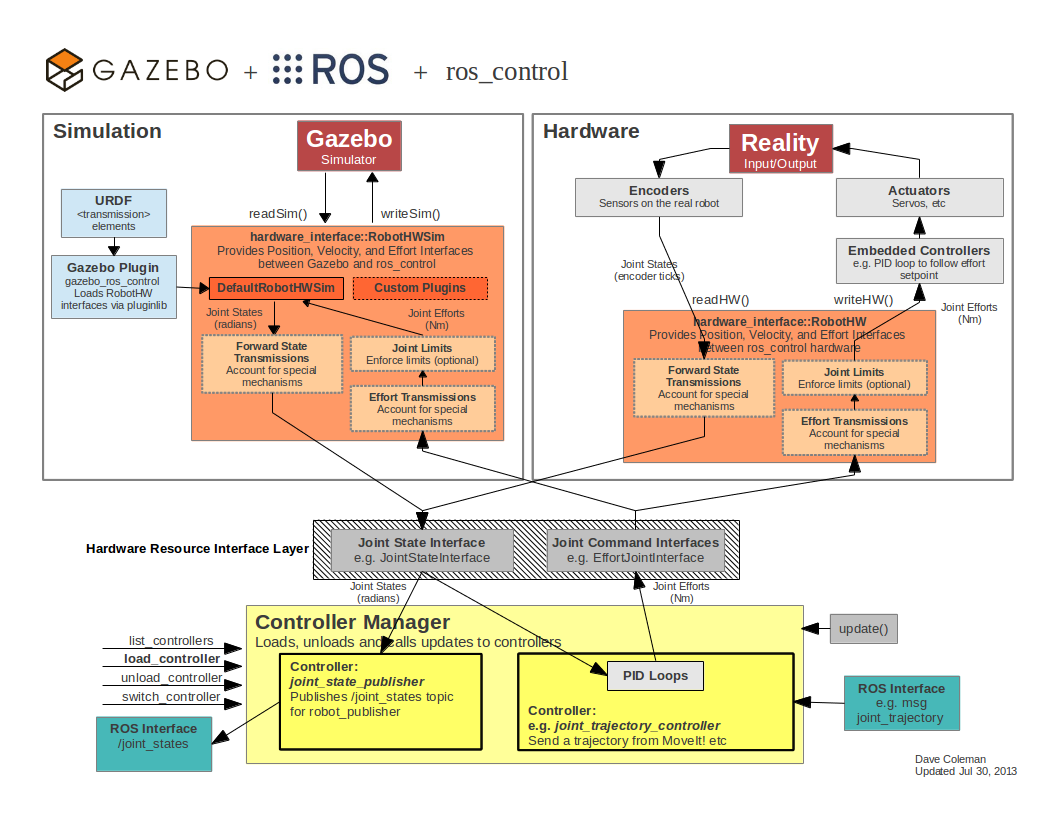
\includegraphics[height=10cm]{img/gazebo_control.png}
        \caption{Gazebo control (Source: \cite{gazebo:ros_control})}
        \label{fig:gazebo_control}
    \end{figure}

    \subsection{RUBI}


\chapter{Documentation of the ROS package stack}

\section{Overview of provided packages}

\section{aleph2\_description}

\section{aleph2\_hardware\_interface}

\section{aleph2\_gazebo}

\section{aleph2\_bringup}

\chapter{Usage}

\chapter{Conclusion}

\bibliographystyle{unsrt}
\bibliography{bibliography}

\end{document}
